\documentclass[11pt,openany]{article}

\usepackage{mathtools, commath}
% Packages for formatting
\usepackage[margin=1in]{geometry}
\usepackage{fancyhdr}
\usepackage{enumerate}
\usepackage{graphicx}
\usepackage{kotex}
\usepackage{amsmath}
\usepackage{amsthm}
\usepackage[dvipsnames,table]{xcolor}
\usepackage{amssymb, amsfonts}

\usepackage{arydshln} % Include this package
% Fonts
\usepackage[T1]{fontenc}
\usepackage[utf8]{inputenc}
\usepackage{newpxtext,newpxmath}
\usepackage{sectsty}

% Define colors
\definecolor{TealBlue1}{HTML}{0077c2}
\definecolor{TealBlue2}{HTML}{00a5e6}
\definecolor{TealBlue3}{HTML}{b3e0ff}
\definecolor{TealBlue4}{HTML}{00293c}
\definecolor{TealBlue5}{HTML}{e6f7ff}

\definecolor{thmcolor}{RGB}{231, 76, 60}
\definecolor{defcolor}{RGB}{52, 152, 219}
\definecolor{lemcolor}{RGB}{155, 89, 182}
\definecolor{corcolor}{RGB}{46, 204, 113}
\definecolor{procolor}{RGB}{241, 196, 15}

\usepackage{color,soul}
\usepackage{soul}
\newcommand{\mathcolorbox}[2]{\colorbox{#1}{$\displaystyle #2$}}
\usepackage{cancel}
\newcommand\crossout[3][black]{\renewcommand\CancelColor{\color{#1}}\cancelto{#2}{#3}}
\newcommand\ncrossout[2][black]{\renewcommand\CancelColor{\color{#1}}\cancel{#2}}

\usepackage{hyperref}
\usepackage{booktabs}

% Chapter formatting
\definecolor{titleTealBlue}{RGB}{0,53,128}
\usepackage{titlesec}
\titleformat{\section}
{\normalfont\sffamily\Large\bfseries\color{titleTealBlue!100!gray}}{\thesection}{1em}{}
\titleformat{\subsection}
{\normalfont\sffamily\large\bfseries\color{titleTealBlue!50!gray}}{\thesubsection}{1em}{}

%Tcolorbox
\usepackage[most]{tcolorbox}
\usepackage{multirow}
\usepackage{multicol}

%Tikzpicture
\usepackage{tikz}
\usepackage{tikz-cd}
\usetikzlibrary{shapes.geometric, calc}
\usetikzlibrary{positioning}
\usetikzlibrary{angles, quotes}
\usetikzlibrary{patterns,patterns.meta}

\usepackage[linesnumbered,ruled]{algorithm2e}
\usepackage{algpseudocode}
\usepackage{setspace}
\SetKwComment{Comment}{/* }{ */}
\SetKwProg{Fn}{Function}{:}{end}
\SetKw{End}{end}
\SetKw{DownTo}{downto}

% Define a new environment for algorithms without line numbers
\newenvironment{algorithm2}[1][]{
	% Save the current state of the algorithm counter
	\newcounter{tempCounter}
	\setcounter{tempCounter}{\value{algocf}}
	% redefine the algorithm numbering (remove prefix)
	\renewcommand{\thealgocf}{}
	\begin{algorithm}
	}{
	\end{algorithm}
	% Restore the algorithm counter state
	\setcounter{algocf}{\value{tempCounter}}
}

\usepackage{adjustbox}
%Tikzpicture
\usepackage{graphicx}
\usepackage{tikz}
\usepackage{tikz-cd}
\usepackage{pgfplots}
\usetikzlibrary{shapes.geometric, calc}
\usetikzlibrary{angles, quotes}
\usetikzlibrary{arrows, arrows.meta}
\usetikzlibrary{patterns,patterns.meta}
\usetikzlibrary{positioning}
\usetikzlibrary{decorations.markings}
\usetikzlibrary{hobby}

%\input{../category-theory-setup-tcolorbox}
% Header and footer formatting
\pagestyle{fancy}
\fancyhead{}
\fancyhf{}
\rhead{\textcolor{TealBlue2}{\textbf{Cryptanalysis-Note}}}%\rule{3cm}{0.4pt}}
\lhead{\textcolor{TealBlue2}{\textbf{Lecture-Note 1}}}
% Define footer
\newcommand{\footer}[1]{
\begin{flushright}
	\vspace{2em}
	
\includegraphics[width=2.5cm]{school_logo.jpg} \\
	\vspace{1em}
	\textcolor{TealBlue2}{\small\textbf{#1}}
\end{flushright}
}
%\rfoot{\large Department of Information Security, Cryptogrphy and Mathematics, Kookmin Uni.
\includegraphics[height=1.5cm]{school_logo.jpg}}
\fancyfoot{}
\fancyfoot[C]{-\thepage-}

\usepackage{amsthm}
\newtheorem{axiom}{Axiom}[section]
\newtheorem{theorem}{Theorem}
\newtheorem*{theorem*}{Theorem}
\newtheorem{proposition}[theorem]{Proposition}
\newtheorem{corollary}{Corollary}[theorem]
\newtheorem*{corollary*}{Corollary}
\newtheorem{lemma}[theorem]{Lemma}
\newtheorem*{lemma*}{Lemma}

\theoremstyle{definition}
\newtheorem{definition}{Definition}
\newtheorem*{definition*}{Definition}
\newtheorem*{note}{Note}
\newtheorem{remark}{Remark}
\newtheorem{example}{Example}
\newtheorem{exercise}{Exercise}[section]
%Tcolorbox
\usepackage[most]{tcolorbox}
\usepackage{varwidth}
\tcbset{colback=white, arc=5pt}

\newtcolorbox{defbox}[2][]{
	enhanced,
	colframe=defcolor, coltitle=white,
	title={\bf #2},#1
}

\newtcolorbox{probox}[2][]{
	enhanced,
	colframe=procolor, coltitle=white,
	title={\bf #2},#1
}


\newtcolorbox{thmbox}[2][]{
	enhanced,
	colframe=thmcolor, coltitle=white,
	title={\bf #2},#1
}

\newtcolorbox{corbox}[2][]{
	enhanced,
	colframe=corcolor, coltitle=white,
	title={\bf #2},#1
}
% Common

\newcommand{\N}{\mathbb{N}}
\newcommand{\Z}{\mathbb{Z}}
\newcommand{\Q}{\mathbb{Q}}
\newcommand{\R}{\mathbb{R}}
\newcommand{\C}{\mathbb{C}}
\newcommand{\F}{\mathbb{F}}

\newcommand{\ie}{\textnormal{i.e.}}
\newcommand{\sol}{\textcolor{magenta}{\bf Sol}}

\newcommand{\inv}[1]{#1^{-1}}
\newcommand{\of}[1]{\left( #1 \right)} 

\newcommand{\uniform}{\overset{\$}{\leftarrow}}
\newcommand{\from}{\leftarrow}

\newcommand{\zero}{\textcolor{red}{\texttt{0}}}
\newcommand{\one}{\textcolor{red}{\texttt{1}}}
\newcommand{\binaryfield}{\set{\zero,\one}}

% for Cryptanalysis

\newcommand{\id}{\textnormal{Id}}
\newcommand{\ddt}{\mathcal{D}}

% for Category Theory

\newcommand{\category}{\mathcal{C}}

\newcommand{\obj}[1]{\mathsf{obj}\left(#1\right)}
\newcommand{\homo}[1]{\mathsf{hom}\left(#1\right)}
\newcommand{\mor}[1]{\mathsf{mor}\left(#1\right)}


\newcommand{\dom}[1]{\mathsf{Dom}\left(#1\right)}
\newcommand{\cdm}[1]{\mathsf{Cdm}\left(#1\right)}

\newcommand{\op}{\textnormal{op}}

% for Lambda Calculus
\newcommand{\src}{\texttt{input}}
\newcommand{\target}{\texttt{output}}
\newcommand{\true}{\mathsf{T}}
\newcommand{\false}{\textsf{F}}

\setstretch{1.25}
\begin{document}
\pagenumbering{arabic}
\begin{center}
	\huge\textbf{Differential Cryptanalysis}\\
	\vspace{0.5em}
	\normalsize{\today}\\
	\vspace{0.5em}
	\large\textbf{Ji, Yong-hyeon}\\x
	\vspace{0.5em}
\end{center}

\section{Definitions}
\subsection{S-Box}
\adjustbox{scale=1.25,center}{
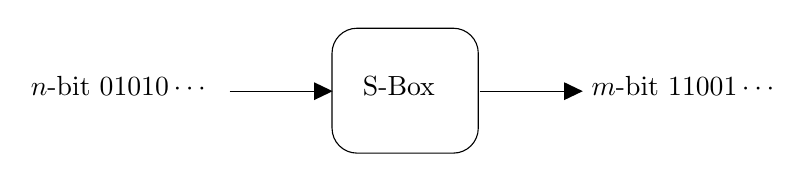
\begin{tikzpicture}[x=0.75pt,y=0.75pt,yscale=-1,xscale=1]
	%uncomment if require: \path (0,300); %set diagram left start at 0, and has height of 300
	
	%Rounded Rect [id:dp9591766320263801] 
	\draw   (319.87,133.03) .. controls (319.87,126.39) and (325.25,121) .. (331.9,121) -- (378.3,121) .. controls (384.95,121) and (390.33,126.39) .. (390.33,133.03) -- (390.33,169.13) .. controls (390.33,175.78) and (384.95,181.17) .. (378.3,181.17) -- (331.9,181.17) .. controls (325.25,181.17) and (319.87,175.78) .. (319.87,169.13) -- cycle ;
	%Straight Lines [id:da23469834338903262] 
	\draw    (270.5,151.33) -- (317.17,151.33) ;
	\draw [shift={(320.17,151.33)}, rotate = 180] [fill={rgb, 255:red, 0; green, 0; blue, 0 }  ][line width=0.08]  [draw opacity=0] (8.93,-4.29) -- (0,0) -- (8.93,4.29) -- cycle    ;
	%Straight Lines [id:da22882668273809115] 
	\draw    (391,151.33) -- (437.67,151.33) ;
	\draw [shift={(440.67,151.33)}, rotate = 180] [fill={rgb, 255:red, 0; green, 0; blue, 0 }  ][line width=0.08]  [draw opacity=0] (8.93,-4.29) -- (0,0) -- (8.93,4.29) -- cycle    ;
	
	% Text Node
	\draw (333.5,142.83) node [anchor=north west][inner sep=0.75pt]   [align=left] {S-Box};
	% Text Node
	\draw (173.5,142.83) node [anchor=north west][inner sep=0.75pt]   [align=left] {$n$-bit $01010\cdots$};
	% Text Node
	\draw (443.67,142.83) node [anchor=north west][inner sep=0.75pt]   [align=left] {$m$-bit $11001\cdots$};	
\end{tikzpicture}}
\vspace{8pt}
\begin{defbox}{S-Box}
\begin{definition}
	Let $n,m\in\Z^+$. A function \[
	S:\F_2^n\to\F_2^m
	\] is a \textbf{S-Box}.
\end{definition}
\end{defbox}

\subsection{The XOR operation}
\[
\fullfunction{\oplus}{\F_2\times\F_2}{\F_2}{(x,y)}{z=x+y\bmod 2}
\]
\begin{center}
	\begin{tabular}{c|c||c}
		\toprule[1.2pt]
		$x$ & $y$ & $z=x\oplus y$\\
		\hline
		0 & 0 & 0\\
		\hline
		0 & 1 & 1\\
		\hline
		1 & 0 & 1\\
		\hline
		1 & 1 & 0\\
		\bottomrule[1.2pt]
	\end{tabular}
\end{center}

\begin{note}[Thinking]
	\[
	\fullfunction{\oplus}{\F_2}{[\F_2\to\F_2]}{x}{\oplus_x=\begin{cases}
			\id(y) &: x=0,\\
			\lnot(y) &: x=1.
	\end{cases}}
	\]
\end{note}


\newpage
\[
\fullfunction{\oplus_n}{\F_2^n\times\F_2^n}{\F_2^n}{\left(\set{x_i}_{i=1}^n,\set{y_i}_{i=1}^n\right)}{\set{x_i\oplus y_i}_{i=1}^n}
\]
\begin{note}
	We use the notation $0_n$ to denote $0_n=(0,\dots,0)$.
\end{note}
\begin{note}[Thinking]
	\[
	\fullfunction{\oplus_n}{\F_2^n}{[\F_2^n\to\F_2^n]}{\set{x_i}_{i=1}^n}{(\oplus_n)_{\set{x_i}_{i=1}^n}=\set{z_i}_{i=1}^n,\ \text{where}\ z_i=\begin{cases}
			\id(y_i) &: x_i=0,\\
			\lnot(y_i) &: x_i=1.
	\end{cases}}
	\]
\end{note}

\begin{probox}{}
\begin{proposition}
	Let $X,Y,Z\in\F_2^n$. Then
	\begin{enumerate}[(1)]
		\item $X\oplus_n Y=Y\oplus_n X$
		\item $(X\oplus_n Y)\oplus Z=X\oplus_n (Y\oplus Z)$
		\item $X\oplus_n 0_n=X=0_n\oplus_n X$
		\item $X\oplus_n X=0_n$
		\item $X\oplus_n Y=0_n\implies X=Y$
		\item $A\oplus_n X=B\implies X=A\oplus_n B$
	\end{enumerate}
\end{proposition}
\end{probox}
\begin{note}
	By $(4)$ and $(5)$, we have $X\oplus_n Y=0\iff X=Y$.
\end{note}
\begin{proof}
	PASS
\end{proof}

\begin{remark}
\ \begin{itemize}
	\item The binary operation $\oplus$ provides the structure of an \textbf{abelian group} on the set $\F_2^n$ with identity element $0_n$.
	\item Because of the property $(4) X\oplus_n X=0_n$, we see that \textit{the inverse of any element is itself} with respect to the operation $\oplus$.
\end{itemize}
\end{remark}

\begin{defbox}{}
	\begin{definition}
		The \textbf{difference} of $X\in\F_2^n$ and $Y\in\F_2^n$ is defined as $X\oplus_n Y\in\F_2^n$.
	\end{definition}
\end{defbox}

\newpage
\section{Difference Set}
\subsection{Definition and Property}
\begin{defbox}{Difference Set of Bit-Sequence}
	\begin{definition}
		Given $\alpha\in\F_2^n$, we define the \textbf{difference set} of $\alpha$ as follow: \[
		\Delta_\alpha=\set{(x_1,x_2)\in\F_2^n\times\F_2^n:x_1\oplus x_2=\alpha\in\F_2^n}\subseteq\F_2^n\times\F_2^n.
		\]
	\end{definition}
\end{defbox}

\begin{probox}{}
\begin{proposition}
	For any $\alpha\in\F_2^n$ the set $\Delta_\alpha$ contains $2^n$ elements and can be expressed as \[
	\Delta_\alpha=\set{(x,x\oplus\alpha):x\in\F_2^n}.
	\]
\end{proposition}
\end{probox}
\begin{proof}
	Let \begin{align*}
		S&:=\set{(x_1,x_2)\in\F_2^n\times\F_2^n:x_1\oplus x_2=\alpha\in\F_2^n}, \\
		T&:=\set{(x,x\oplus\alpha):x\in\F_2^n}.
	\end{align*} We must show that $S=T$:
	\begin{itemize}
		\item[] ($S\subseteq T$) Let $(x,y)\in S$ then by definition $x\oplus y=\alpha$.
		Since $(x\oplus y=\alpha)\Rightarrow (y=x\oplus \alpha)$, \[
		(x,y)=(x,x\oplus \alpha)\in T.
		\]
		\item[]($T\subseteq S$) Let $(x,x\oplus\alpha)\in T$. Since \[
		x\oplus(x\oplus\alpha)=\alpha,
		\] $(x,x\oplus\alpha)\in S$.
	\end{itemize}
\end{proof}
\begin{corbox}{}
\begin{corollary}
	For any $\alpha\in\F_2^n$, we have $\Delta_\alpha\simeq \F_2^n$.
\end{corollary}
\end{corbox}
\begin{remark}
Let us consider the case $\alpha=0$ for the set $\Delta_\alpha$. When $\alpha=0$ the difference set is \[
\Delta_0=\set{(x,x):x\in\F_2^n}
\] This set is often called the \textbf{diagonal} of $\F_2^n\times\F_2^n$.
\end{remark}

\newpage
\subsection{Difference Sets of a S-BOX}
\adjustbox{scale=.9,center}{
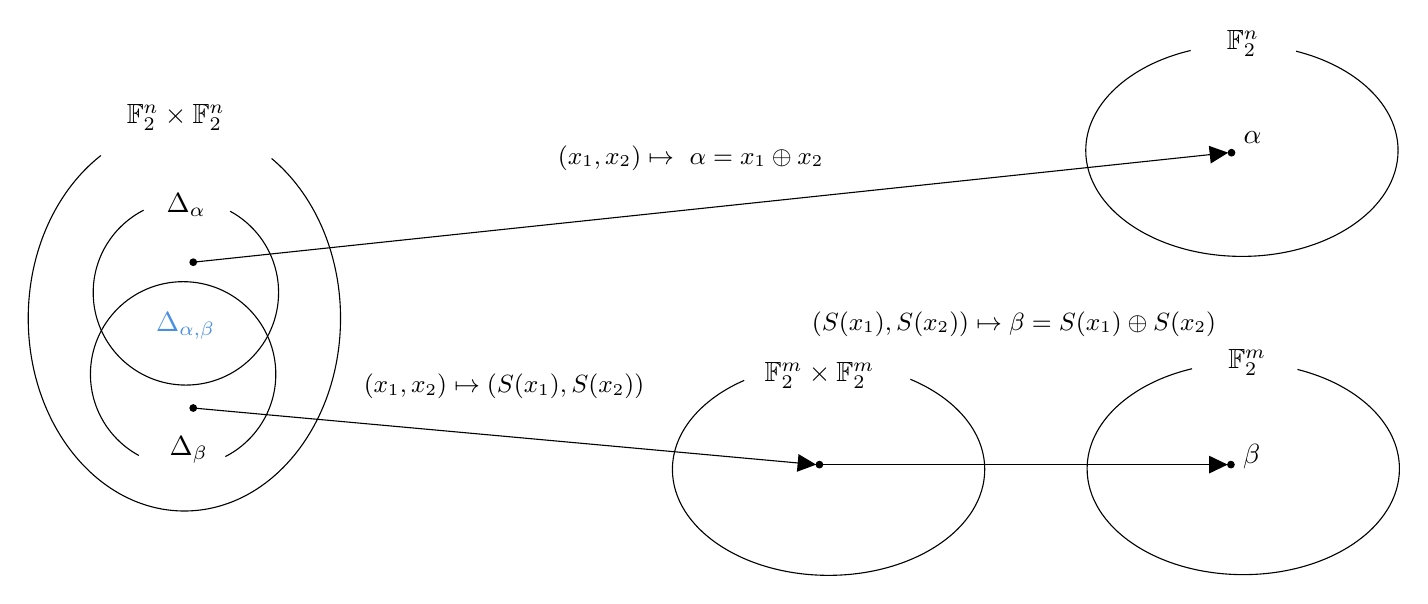
\begin{tikzpicture}[x=0.75pt,y=0.75pt,yscale=-1,xscale=1]
	%uncomment if require: \path (0,300); %set diagram left start at 0, and has height of 300
	
	%Shape: Arc [id:dp8485446560706211] 
	\draw  [draw opacity=0] (137.79,79.83) .. controls (157.82,96.51) and (171,124.78) .. (171,156.84) .. controls (171,208.11) and (137.32,249.67) .. (95.77,249.67) .. controls (54.22,249.67) and (20.53,208.11) .. (20.53,156.84) .. controls (20.53,123.83) and (34.5,94.84) .. (55.55,78.38) -- (95.77,156.84) -- cycle ; \draw   (137.79,79.83) .. controls (157.82,96.51) and (171,124.78) .. (171,156.84) .. controls (171,208.11) and (137.32,249.67) .. (95.77,249.67) .. controls (54.22,249.67) and (20.53,208.11) .. (20.53,156.84) .. controls (20.53,123.83) and (34.5,94.84) .. (55.55,78.38) ;  
	%Shape: Arc [id:dp8649167287391757] 
	\draw  [draw opacity=0] (117.85,105.27) .. controls (131.73,112.83) and (141.15,127.53) .. (141.15,144.42) .. controls (141.15,169.04) and (121.15,189) .. (96.49,189) .. controls (71.83,189) and (51.83,169.04) .. (51.83,144.42) .. controls (51.83,127.12) and (61.71,112.12) .. (76.14,104.73) -- (96.49,144.42) -- cycle ; \draw   (117.85,105.27) .. controls (131.73,112.83) and (141.15,127.53) .. (141.15,144.42) .. controls (141.15,169.04) and (121.15,189) .. (96.49,189) .. controls (71.83,189) and (51.83,169.04) .. (51.83,144.42) .. controls (51.83,127.12) and (61.71,112.12) .. (76.14,104.73) ;  
	%Shape: Arc [id:dp7550356773071991] 
	\draw  [draw opacity=0] (73.79,222.91) .. controls (59.91,215.35) and (50.5,200.65) .. (50.5,183.76) .. controls (50.5,159.14) and (70.49,139.18) .. (95.16,139.18) .. controls (119.82,139.18) and (139.81,159.14) .. (139.81,183.76) .. controls (139.81,201.06) and (129.94,216.06) .. (115.5,223.45) -- (95.16,183.76) -- cycle ; \draw   (73.79,222.91) .. controls (59.91,215.35) and (50.5,200.65) .. (50.5,183.76) .. controls (50.5,159.14) and (70.49,139.18) .. (95.16,139.18) .. controls (119.82,139.18) and (139.81,159.14) .. (139.81,183.76) .. controls (139.81,201.06) and (129.94,216.06) .. (115.5,223.45) ;  
	%Shape: Arc [id:dp14104992338992095] 
	\draw  [draw opacity=0] (631.38,28.14) .. controls (660.06,35.34) and (680.51,54.05) .. (680.51,75.99) .. controls (680.51,104.16) and (646.82,127) .. (605.27,127) .. controls (563.72,127) and (530.04,104.16) .. (530.04,75.99) .. controls (530.04,53.69) and (551.15,34.73) .. (580.57,27.8) -- (605.27,75.99) -- cycle ; \draw   (631.38,28.14) .. controls (660.06,35.34) and (680.51,54.05) .. (680.51,75.99) .. controls (680.51,104.16) and (646.82,127) .. (605.27,127) .. controls (563.72,127) and (530.04,104.16) .. (530.04,75.99) .. controls (530.04,53.69) and (551.15,34.73) .. (580.57,27.8) ;  
	%Shape: Arc [id:dp20130572401760238] 
	\draw  [draw opacity=0] (632.05,181.47) .. controls (660.73,188.67) and (681.17,207.38) .. (681.17,229.33) .. controls (681.17,257.5) and (647.49,280.33) .. (605.94,280.33) .. controls (564.39,280.33) and (530.7,257.5) .. (530.7,229.33) .. controls (530.7,207.02) and (551.82,188.06) .. (581.23,181.13) -- (605.94,229.33) -- cycle ; \draw   (632.05,181.47) .. controls (660.73,188.67) and (681.17,207.38) .. (681.17,229.33) .. controls (681.17,257.5) and (647.49,280.33) .. (605.94,280.33) .. controls (564.39,280.33) and (530.7,257.5) .. (530.7,229.33) .. controls (530.7,207.02) and (551.82,188.06) .. (581.23,181.13) ;  
	%Shape: Circle [id:dp7486206290599853] 
	\draw  [fill={rgb, 255:red, 0; green, 0; blue, 0 }  ,fill opacity=1 ] (598.68,77.04) .. controls (598.68,76.17) and (599.39,75.46) .. (600.26,75.46) .. controls (601.14,75.46) and (601.84,76.17) .. (601.84,77.04) .. controls (601.84,77.91) and (601.14,78.62) .. (600.26,78.62) .. controls (599.39,78.62) and (598.68,77.91) .. (598.68,77.04) -- cycle ;
	%Shape: Circle [id:dp2708432240553855] 
	\draw  [fill={rgb, 255:red, 0; green, 0; blue, 0 }  ,fill opacity=1 ] (598.4,227.32) .. controls (598.4,226.45) and (599.11,225.74) .. (599.98,225.74) .. controls (600.85,225.74) and (601.56,226.45) .. (601.56,227.32) .. controls (601.56,228.2) and (600.85,228.9) .. (599.98,228.9) .. controls (599.11,228.9) and (598.4,228.2) .. (598.4,227.32) -- cycle ;
	%Straight Lines [id:da6402831064609027] 
	\draw    (100.03,129.8) -- (595.7,77.35) ;
	\draw [shift={(598.68,77.04)}, rotate = 173.96] [fill={rgb, 255:red, 0; green, 0; blue, 0 }  ][line width=0.08]  [draw opacity=0] (8.93,-4.29) -- (0,0) -- (8.93,4.29) -- cycle    ;
	%Shape: Arc [id:dp5106575548043777] 
	\draw  [draw opacity=0] (445.54,186.2) .. controls (467.04,195.18) and (481.37,211.28) .. (481.37,229.66) .. controls (481.37,257.83) and (447.69,280.67) .. (406.14,280.67) .. controls (364.59,280.67) and (330.9,257.83) .. (330.9,229.66) .. controls (330.9,211.64) and (344.69,195.8) .. (365.51,186.72) -- (406.14,229.66) -- cycle ; \draw   (445.54,186.2) .. controls (467.04,195.18) and (481.37,211.28) .. (481.37,229.66) .. controls (481.37,257.83) and (447.69,280.67) .. (406.14,280.67) .. controls (364.59,280.67) and (330.9,257.83) .. (330.9,229.66) .. controls (330.9,211.64) and (344.69,195.8) .. (365.51,186.72) ;  
	%Straight Lines [id:da7185466059100425] 
	\draw    (401.73,227.32) -- (595.4,227.32) ;
	\draw [shift={(598.4,227.32)}, rotate = 180] [fill={rgb, 255:red, 0; green, 0; blue, 0 }  ][line width=0.08]  [draw opacity=0] (8.93,-4.29) -- (0,0) -- (8.93,4.29) -- cycle    ;
	%Straight Lines [id:da12390164887496624] 
	\draw    (100.03,200.05) -- (397.16,227.05) ;
	\draw [shift={(400.15,227.32)}, rotate = 185.19] [fill={rgb, 255:red, 0; green, 0; blue, 0 }  ][line width=0.08]  [draw opacity=0] (8.93,-4.29) -- (0,0) -- (8.93,4.29) -- cycle    ;
	%Shape: Circle [id:dp7469134159387805] 
	\draw  [fill={rgb, 255:red, 0; green, 0; blue, 0 }  ,fill opacity=1 ] (400.15,227.32) .. controls (400.15,226.45) and (400.86,225.74) .. (401.73,225.74) .. controls (402.6,225.74) and (403.31,226.45) .. (403.31,227.32) .. controls (403.31,228.2) and (402.6,228.9) .. (401.73,228.9) .. controls (400.86,228.9) and (400.15,228.2) .. (400.15,227.32) -- cycle ;
	%Shape: Circle [id:dp892233202904773] 
	\draw  [fill={rgb, 255:red, 0; green, 0; blue, 0 }  ,fill opacity=1 ] (98.45,200.05) .. controls (98.45,199.17) and (99.16,198.47) .. (100.03,198.47) .. controls (100.91,198.47) and (101.61,199.17) .. (101.61,200.05) .. controls (101.61,200.92) and (100.91,201.63) .. (100.03,201.63) .. controls (99.16,201.63) and (98.45,200.92) .. (98.45,200.05) -- cycle ;
	%Shape: Circle [id:dp961142920919116] 
	\draw  [fill={rgb, 255:red, 0; green, 0; blue, 0 }  ,fill opacity=1 ] (98.45,129.8) .. controls (98.45,128.92) and (99.16,128.22) .. (100.03,128.22) .. controls (100.91,128.22) and (101.61,128.92) .. (101.61,129.8) .. controls (101.61,130.67) and (100.91,131.38) .. (100.03,131.38) .. controls (99.16,131.38) and (98.45,130.67) .. (98.45,129.8) -- cycle ;
	
	% Text Node
	\draw (66.77,52.73) node [anchor=north west][inner sep=0.75pt]    {$\F_{2}^{n} \times \F_{2}^{n}$};
	% Text Node
	\draw (85.98,95.35) node [anchor=north west][inner sep=0.75pt]    {$\Delta _{\alpha }$};
	% Text Node
	\draw (87.44,212.4) node [anchor=north west][inner sep=0.75pt]    {$\Delta _{\beta }$};
	% Text Node
	\draw (80.92,152.77) node [anchor=north west][inner sep=0.75pt]  [color={rgb, 255:red, 74; green, 144; blue, 226 }  ,opacity=1 ]  {$\Delta _{\alpha ,\beta }$};
	% Text Node
	\draw (596.77,17.07) node [anchor=north west][inner sep=0.75pt]    {$\F_{2}^{n}$};
	% Text Node
	\draw (597.44,170.4) node [anchor=north west][inner sep=0.75pt]    {$\F_{2}^{m}$};
	% Text Node
	\draw (604.86,65.73) node [anchor=north west][inner sep=0.75pt]    {$\alpha $};
	% Text Node
	\draw (604.57,216.02) node [anchor=north west][inner sep=0.75pt]    {$\beta $};
	% Text Node
	\draw (374.1,176.73) node [anchor=north west][inner sep=0.75pt]    {$\F_{2}^{m} \times \F_{2}^{m}$};
	% Text Node
	\draw (274.43,72.23) node [anchor=north west][inner sep=0.75pt]  [font=\small]  {$( x_{1} ,x_{2}) \mapsto \ \alpha =x_{1} \oplus x_{2}$};
	% Text Node
	\draw (180.93,182.23) node [anchor=north west][inner sep=0.75pt]  [font=\small]  {$( x_{1} ,x_{2}) \mapsto ( S( x_{1}) ,S( x_{2}))$};
	% Text Node
	\draw (396.83,152.23) node [anchor=north west][inner sep=0.75pt]  [font=\small]  {$( S( x_{1}) ,S( x_{2})) \mapsto \beta =S( x_{1}) \oplus S( x_{2})$};
\end{tikzpicture}}
\vspace{12pt}
\begin{defbox}{Difference Set of a S-BOX}
Let $S:\F_2^n\to\F_2^m$ is a S-box. Let $\alpha\in\F_2^n$ and $\beta\in\F_2^m$. Consider \begin{align*}
	\Delta_\alpha&=\set{(x_1,x_2):x_1\oplus x_2=\alpha\in\F_2^n}\subseteq\F_2^n\times\F_2^n\quad \text{and}\\
	\Delta_\beta&=\set{(x_1,x_2):S(x_1)\oplus S(x_2)=\beta\in\F_2^m}\subseteq\F_2^n\times\F_2^n.
\end{align*}
We define the \textbf{difference set} of $S$ with respect to $\alpha$ and $\beta$ by \[
\Delta_{\alpha,\beta}=\Delta_\alpha\cap\Delta_\beta=\set{(x_1,x_2)\in\F_2^n\times\F_2^n:x_1\oplus x_2=\alpha\in\F_2^n\ \text{and}\ S(x_1)\oplus S(x_2)=\beta\in\F_2^m}.
\] That is, $\Delta_{\alpha,\beta}$ is the set of ordered pairs of elements from $\F_2^n$ which have a difference of $\alpha$ and such that their images under $S$ have a difference of $\beta$.
\end{defbox}
\begin{remark}
\ \begin{itemize}
	\item This can also written as \[
	\Delta_{\alpha,\beta}=\set{(x_1,x_2)\in\Delta_\alpha:(S(x_1),S(x_2))\in\Delta_\beta}.
	\]
	\item $\Delta_{\alpha,\beta}$ is always defined w.r.t. a given S-Box $S$. If we want to make this dependence explicit we can write $\Delta_{\alpha,\beta}^S$.
\end{itemize}
\end{remark}
\vspace{12pt}
\begin{defbox}{Cardinality of a Difference Set}
	We define $\delta_{\alpha,\beta}$ to be the cardinality of the finite set $\Delta_{\alpha,\beta}$, namely \[
	\delta_{\alpha,\beta}:=\abs{\Delta_{\alpha,\beta}}\in\Z_{\geq 0}.
	\]
\end{defbox}

\vspace{12pt}
\begin{probox}{}
	\begin{proposition}
		\[
		\delta_{\alpha,\beta}=\#\set{x\in\F_2^n:S(x)\oplus S(x\oplus\alpha)=\beta\in\F_2^m}.
		\]
	\end{proposition}
\end{probox}
\begin{proof}
	\begin{align*}
		\Delta_{\alpha ,\beta }=\Delta_{\alpha}\cap\Delta_{\beta}
		&=\set{(x_1,x_2):x_1\oplus x_2=\alpha}\cap \set{(x_1,x_2):S(x_1)\oplus S(x_2)=\beta}\\
		&=\set{(x,x\oplus\alpha):x\in\F_2^n}\cap \set{(x_1,x_2):S(x_1)\oplus S(x_2)=\beta} \\
		&=\set{x\in\F_2^n:S(x)\oplus S(x\oplus \alpha)=\beta\in\F_2^m}.
	\end{align*}
\end{proof}

\begin{remark}
\ \begin{itemize}
	\item When $\alpha=0$ and $\beta=0$ we have
	$\Delta_{0,0}=\Delta_0=\set{(x,x):x\in\F_2^n}$.
	\item In general when $\alpha=0$ we find that
	$\Delta_{0,\beta}=\begin{cases}
		\Delta_0 &:\beta=0\\
		\emptyset &:\beta\neq 0
	\end{cases}$
	\item  Since $\abs{\Delta_0}=2^n$ and $\abs{\emptyset}=0$,\quad
	$\delta_{0,\beta}=\begin{cases}
		2^n &:\beta=0 \\
		0 &:\beta\neq 0
	\end{cases}$.
\end{itemize}
\end{remark}

\begin{probox}{}
	\begin{proposition}
		The integer $\delta_{\alpha,\beta}\in\Z_{\geq 0}$ is always even.
	\end{proposition}
\end{probox}
\begin{proof}
	Recall that $0$ is even.
	\begin{itemize}
		\item[] (Case I) When $\alpha=0$, we saw either $\delta_{0,\beta}\in\set{0,2^n}$ and these are even in either case.
		\item[] (Case II) Suppose that $\alpha\neq 0$ and $\Delta_{\alpha,\beta}\neq\emptyset$. Let $(x_1,x_2)\in\Delta_{\alpha,\beta}$ then \[
		(x_2,x_1)\in\Delta_{\alpha,\beta}\quad\text{and}\quad x_1\neq x_2.
		\] Therefore $(x_1,x_2)\neq(x_2,x_1)$. So if we pair $(x_1,x_2)$ and $(x_2,x_1)$, we can partition $\Delta_{\alpha,\beta}$ into subsets, each subset having cardinality of $2$.
	\end{itemize}
\end{proof}

\section{The DDT of a S-Box}
\subsection{Definition and Property}

\begin{defbox}{Differential Distribution Table}
Let $S:\F_2^n\to\F_2^m$ be a S-Box. The \textbf{differential distribution table} (abbreviated DDT) of $S$
is a table (or matrix) with $2^n$-rows and $2^m$-columns. We denote it by $\mathcal{D}_S$ or just by $\mathcal{D}$.
\begin{itemize}
	\item The rows are indexed by the elements $\alpha\in\F_2^n=\set{0,\dots,2^n-1}$.
	\item The columns are indexed by the elements $\beta\in\F_2^m=\set{0,\dots,2^m-1}$.
	\item The entry at row index $\alpha$ and column index $\beta$ is given by $\delta_{\alpha,\beta}=\abs{\Delta_{\alpha,\beta}}$. That is, \[
	\mathcal{D}=(\delta_{\alpha,\beta})_{2^n\times 2^m}.
	\] 
\end{itemize}
\end{defbox}
\begin{remark}
The DDT of a S-Box is just table of all the possible integer values  $\delta_{\alpha,\beta}$.
\begin{table}[h!]\centering
	\renewcommand{\arraystretch}{1.25}
	\begin{tabular}{c||cccccc}
		$\mathcal{D}$ & 0 & 1 & $\cdots$ & $\beta$ & $\cdots$ & $2^{m}-1$\\
		\hline
		\hline
		0 & $2^{n}$ & 0 & &$\cdots$ & & 0 \\
		1 &  \\
		$\vdots$ &  \\
		$\alpha$ &  & & & $\delta_{\alpha,\beta}$& \\
		$\vdots$ & \\
		$2^n-1$ &  \\
	\end{tabular}
\end{table}
\end{remark}
\vspace{12pt}
\begin{probox}{}
\begin{proposition}
Let $S:\F_2^n\to\F_2^m$ be a S-Box with differential distribution table $\ddt$. The following properties hold for $\ddt$. \begin{enumerate}[(1)]
	\item Every entry in $\ddt$ is a non-negative even integer between $0$ and $2^n$.
	\item The top-left entry of $\ddt$ is $2^n$.
	\item The first row of $\ddt$ consists of all zeros except the first entry which is $2^n$.
	\item If $S$ is one-to-one then the first column of $\ddt$ consists all zeros except the first entry which is $2^n$.
	\item The sum of the entries of each row is $2^n$.
	\item If $S$ is bijective then every row and column of the DDT add up to $2^n$.
\end{enumerate}
\end{proposition}
\end{probox}

\newpage
\subsection{The DDT and Probabilities}
When designing and analyzing attacks by differential cryptanalysis, we often want to translate the integer values from the DDT into probabilities.

\begin{note}
The \textbf{probability} $p$ that $E$ occurs is defined to be the quotient of the cardinalities of the sets $E$ and $\Omega$: \[
p=\frac{\abs{E}}{\abs{\Omega}}.
\]
\end{note}

\begin{defbox}{Probability of DDT}
\begin{definition}
	Let the universe is $\Omega=\Delta_\alpha$ and the event $E=\Delta_{\alpha,\beta}$. We define probability $p_{\alpha,\beta}$ as follows: \[
	p_{\alpha,\beta}=\frac{\abs{\Delta_{\alpha,\beta}}}{\abs{\Delta_\alpha}}=\frac{\delta_{\alpha,\beta}}{2^n}.
	\]
\end{definition}
\end{defbox}
\begin{remark}
	Equivalently we can regard the universe $\Omega=\F_2^n$ and the event as the set \[
	E=\set{x\in\F_2^n:S(x)\oplus S(x\oplus\alpha)=\beta}.
	\]
\end{remark}

\section{The DDT of a Linear S-Box}
\begin{defbox}{Linear S-Box}
\begin{definition}
A S-Box $L:\F_2^n\to\F_2^m$ is said to be \textbf{linear} if \[
x_1,x_2\in\F_2^n\implies L(x_1\oplus x_2)=L(x_1)\oplus L(x_2).
\]
\end{definition}
\end{defbox}
\vspace{12pt}
\begin{probox}{}
\begin{proposition}
Let $L:\F_2^n\to\F_2^m$ be a linear S-Box. Let $\alpha\in\F_2^n$ and $\beta\in\F_2^n$. Then the difference sets of $L$ and their cardinalities are given by \[
\Delta_{\alpha,\beta}=\begin{cases}
\Delta_\alpha &:\beta=L(\alpha)\\
\emptyset &:\beta\neq L(\alpha)
\end{cases},\quad \delta_{\alpha,\beta}=\begin{cases}
2^n &:\beta=L(\alpha)\\
0 &:\beta\neq L(\alpha)
\end{cases}.
\] That is, every row of the DDT of $L$ consists of all zeros except one entry with a value of $2^n$.
\end{proposition}
\end{probox}
\begin{proof}
	Let $\alpha\in\F_2^n$. Assume that $(x_1,x_2)\in\Delta_{\alpha}$, namely $x_1\oplus x_2=\alpha$ then \[
	L(x_1)\oplus L(x_2)=L(x_1\oplus x_2)=L(\alpha).
	\] So $(x_1,x_2)\in\Delta_{\alpha,\beta}\iff\beta=L(\alpha)$.
\end{proof}

\footer{Department of Information Security, Cryptology and Mathematics\\
	College of Science and Technology\\
	Kookmin University}

\newpage
\begin{thebibliography}{99}
	
%\bibitem{schlenga2020cdcl}
%Schlenga, Alexander T. (2020). "Conflict Driven Clause Learning". June 8, 2020.

\bibitem{youtube_intro_to_category_theory}
``Intro to Category Theory'' YouTube, uploaded by Warwick Mathematics Exchange, 1 Feb 2023, \url{https://www.youtube.com/watch?v=AUD2Rpoy6O4}

\bibitem{proofwiki_definition_metacategory}
ProofWiki. ``Definition:Metacategory'' Accessed on [May 05, 2024]. \url{https://proofwiki.org/wiki/Definition:Metacategory}.

\bibitem{nLab_category}
nLab. ``category'' Accessed on [May 05, 2024]. \url{https://ncatlab.org/nlab/show/category#Grothendieck61}.
% Add all the references in the same way
% Use \bibitem for each reference
	
\end{thebibliography}
%\bibliography{category-theory-note-ref}
%\bibliographystyle{abbrv}
\end{document}